% !Mode:: "TeX:UTF-8"
%\chapter{预备知识}
%\label{chap:java_knowledges}


%文章一个回车不会分段,可自由编写。
本书有四部分组成,重点学习Java的编程基础。
机器学习是本书的一大特色,帮助同学们在学习Java的同时也能掌握一些人工智能的知识。
现在很多大学甚至中学都开设了机器学习的课程,可见是非常流行,也是大众都能接受的一门知识。
虽然涉及到很多数学推理,但对于应用型的人群来说,了解其原理学会使用并不复杂。
目前,已有很多成熟的算法模型可以使用。
下\figref{fig:part1_scikit_algo}引自scikit-learn。

\begin{figure}[!htb]
	\centerline{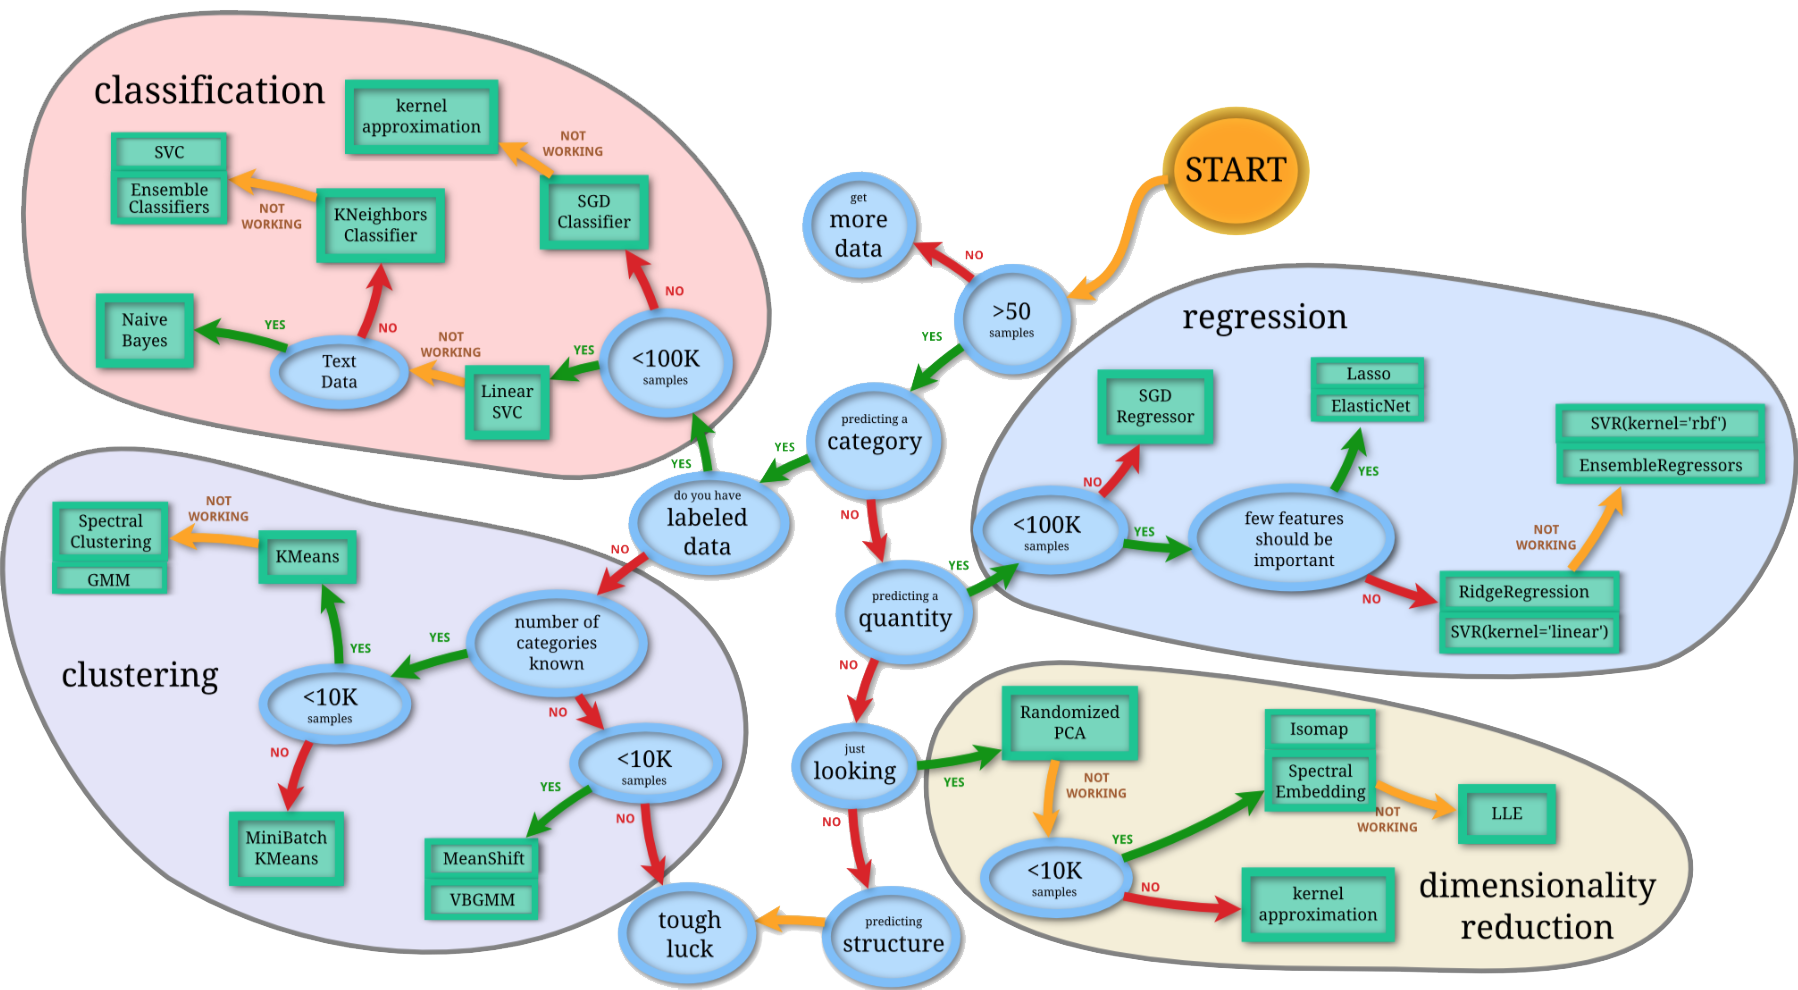
\includegraphics[width=.5\figwidth]{images/scikit-algo.png}}
	\caption{问题分类}
	\label{fig:part1_scikit_algo}
\end{figure}

机器学习(Machine Learning, ML)是一门多领域交叉学科,涉及概率论、统计学、逼近论、凸分析、算法复杂度理论等多门学科。
专门研究计算机怎样模拟或实现人类的学习行为,以获取新的知识或技能重新组织已有的知识结构使之不断改善自身的性能。
人类对于大脑的研究,始于计算机诞生之前。而在计算机问世以后,对人工智能的研究掀起了一次次浪潮。
直到21世纪,这股浪潮席卷了各个领域,人工智能理论也愈加成熟。借助计算机能解决的问题越来越多,变得越来越智能化。
计算机从诞生,就被赋予了人工智能的希望。

上个世纪,图灵提出了一个判断计算机是否具备智能的测试标准。测试者与被测试者(一个人和一台机器)隔开的情况下,通过一些装置(如键盘)向被测试者随意提问。进行多次测试后,如果有超过30\%的测试者不能确定出被测试者是人还是机器,那么这台机器就通过了测试,并被认为具有人类智能。
\figref{fig:part1_turning_test}展示了这样一个场景。

\begin{figure}[!htb]
\centerline{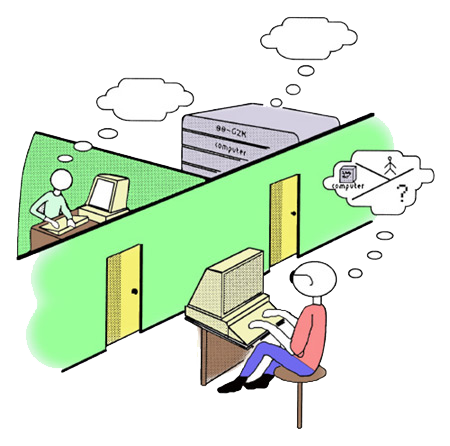
\includegraphics[width=.3\figwidth]{images/turingtest.png}}
\caption{图灵测试}
\label{fig:part1_turning_test}
\end{figure}

本章作为Java学习的入门基础篇,将为大家逐步揭开Programmaing的奥秘。也许,你有很多关于计算机的疑问,请仔细阅读本章相关的内容,相信你必有所获!如若你已具备Java编程知识,你可以大胆地跳过本章。但我建议看看也无妨,毕竟Java语言出现了很多变化。